\section{Flow in an array of charged squares}

In this section, flow through a periodic structure is modelled. The
structure is consists of squares placed in a periodic pattern shown in
fig. \ref{fig:res:square}. The unit cell, used in the computation is
marked by the dashed box in the figure. The dimension of the unit cell
is chosen to $10 \mu$m and the permeability through the structure is
investigated for different sizes of the squares. Also the effect of
having charged vs. uncharged squares is studied. 

In fig. \ref{fig:res:s_uncharged} and fig. \ref{fig:res:s_charged} the
computed velocity fields around a square in a unit cell is
visualised. The side of the square is of length $0.5d$.   

\begin{figure}
  \centering
  \subfloat[Velocity field
    ]{\label{fig:res:hetasdro}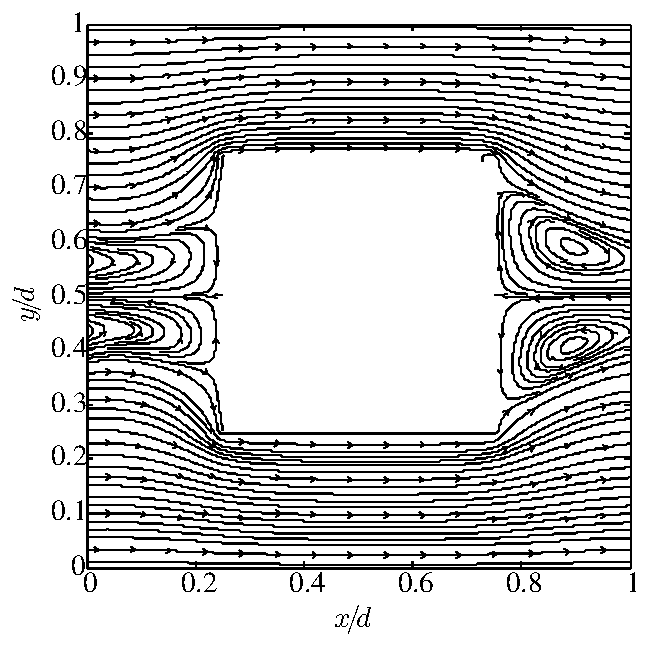
\includegraphics[width=0.47\textwidth]{fig/s_field_uncharged.pdf}}      
  \hspace{5pt} \subfloat[$|\ubf|$
  ]{\label{fig:res:squasadre}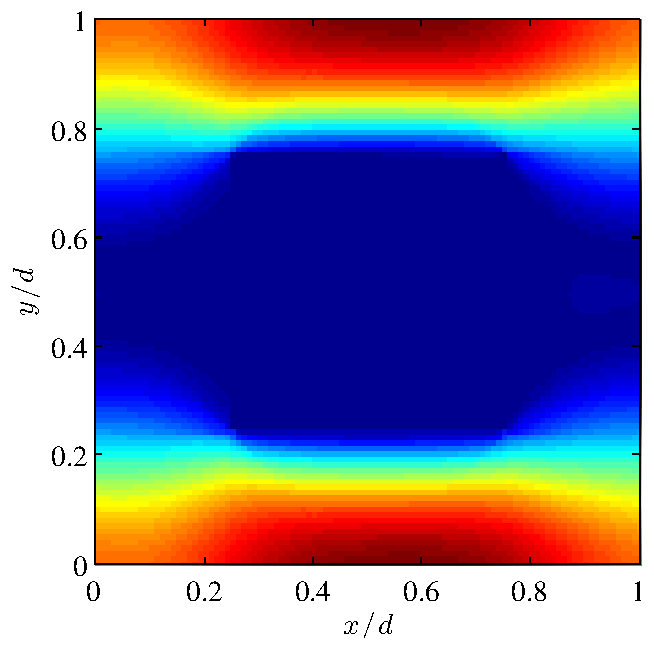
\includegraphics[width=0.47\textwidth]{fig/s_u_uncharged.pdf}}
  \caption[Velocity field for flow through an array of
    uncharged squares.]{Visualised velocity field for flow
    through an array of \textbf{uncharged} squares. The magnitude of
    the velocity varies between 0.20 m/s (red) to 0 m/s (blue).}
  \label{fig:res:s_uncharged}
\end{figure}


\begin{figure}
  \centering
  \subfloat[Velocity field
    ]{\label{fig:res:asas}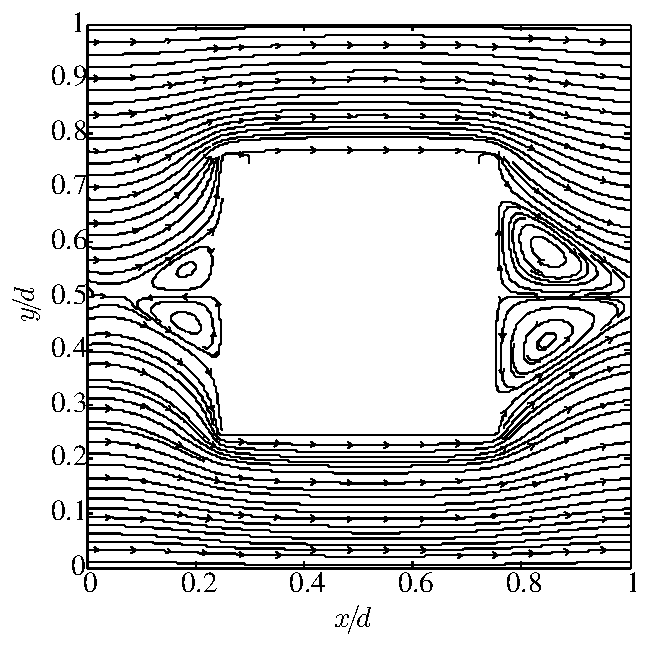
\includegraphics[width=0.47\textwidth]{fig/s_field_charged.pdf}}      
  \hspace{5pt} \subfloat[$|\ubf|$
  ]{\label{fig:res:asdda}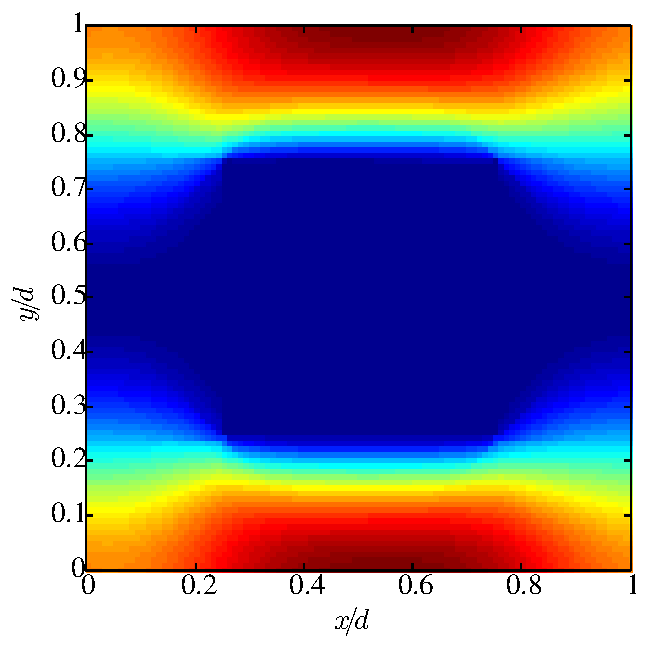
\includegraphics[width=0.47\textwidth]{fig/s_u_charged.pdf}}
  \caption[Velocity field for flow through an array of charged
    squares.]{Visualised velocity field for flow through an array of
    \textbf{charged} squares. The magnitude of the velocity varies
    between 0.16 m/s (orange) to 0 m/s (blue). The surface charge is
    set to $\sigma_s = 1.78 \mu$C/m$^2$. The same colour scale as is
  fig. \ref{fig:res:s_uncharged} is used.}
  \label{fig:res:s_charged}
\end{figure}

The main effect noted that the charge on the square has on the flow,
is that it is slowed down. This is due to that charge inhomogeneities
arise when the charged square is introduced and from this the flow is
slowed down due to the electroviscous effect. In
figs. \ref{fig:res:mid} and \ref{fig:res:pre}, the velocity component
in the pressure drop direction (x) is shown in a section at $x = d/2$
and $x = 0$ respectively.  

\begin{figure}
\begin{center}
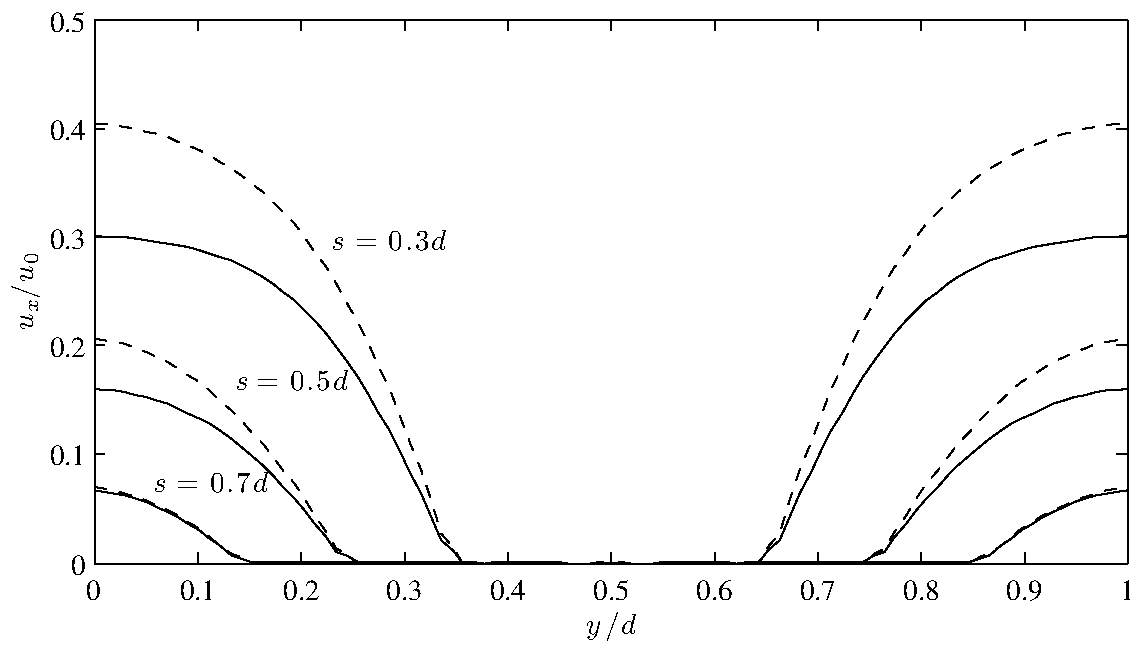
\includegraphics[width=0.9\textwidth]{fig/square_u_mid.pdf}
\end{center}
\caption[Section of the velocity field through a square
  array.]{Velocity profiles across the square array at $x = d/2$ in
  the cell. The sides of the squares are varied between $0.3d$, $0.5d$
  and $0.7d$ where $d = 10 \mu$m is the length of the cell. The flow
  is driven by a pressure gradient and the uncharged (dashed) and
  charged (solid) squares are compared. $\sigma_s = 1.78 \mu$C/m$^2$
  (solid), $\partial_xP = 0.5$ kPa/m and $u_0 = 1$ mm/s. }
\label{fig:res:mid}
\end{figure}

\begin{figure}
\begin{center}
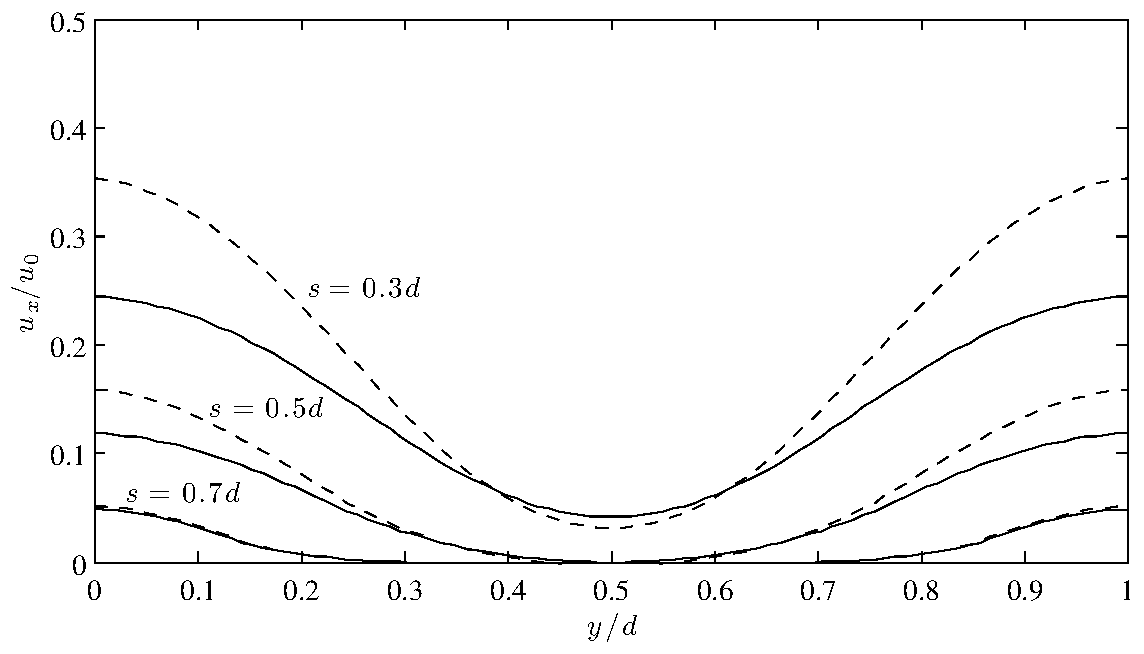
\includegraphics[width=0.9\textwidth]{fig/square_pre_u.pdf}
\end{center}
\caption[Section of the velocity field through a square
  array.]{Velocity profiles across the square array at $x = 0$ in the
  cell. The sides of the squares are varied between $0.3d$, $0.5d$ and
  $0.7d$ where $d = 10 \mu$m is the length of the cell. The flow is
  driven by a pressure gradient and the uncharged (dashed) and charged
  (solid) squares are compared. $\sigma_s = 1.78 \mu$C/m$^2$ (solid),
  $\partial_xP = 0.5$ kPa/m and $u_0 = 1$ mm/s. }
\label{fig:res:pre}
\end{figure}
